\documentclass{article}

\usepackage{graphicx}
\usepackage{tikz}
\usepackage{tikzsymbols}
\usetikzlibrary{calc,patterns,shapes.geometric}
\pagestyle{empty}
\usepackage[margin=0pt]{geometry}
\geometry{papersize={14in,12in}}

\def\centerarc[#1](#2)(#3:#4:#5){\draw[#1] ($(#2)+({#5*cos(#3)},{#5*sin(#3)})$) arc (#3:#4:#5);}

\begin{document}
	\begin{figure}
		\centering
		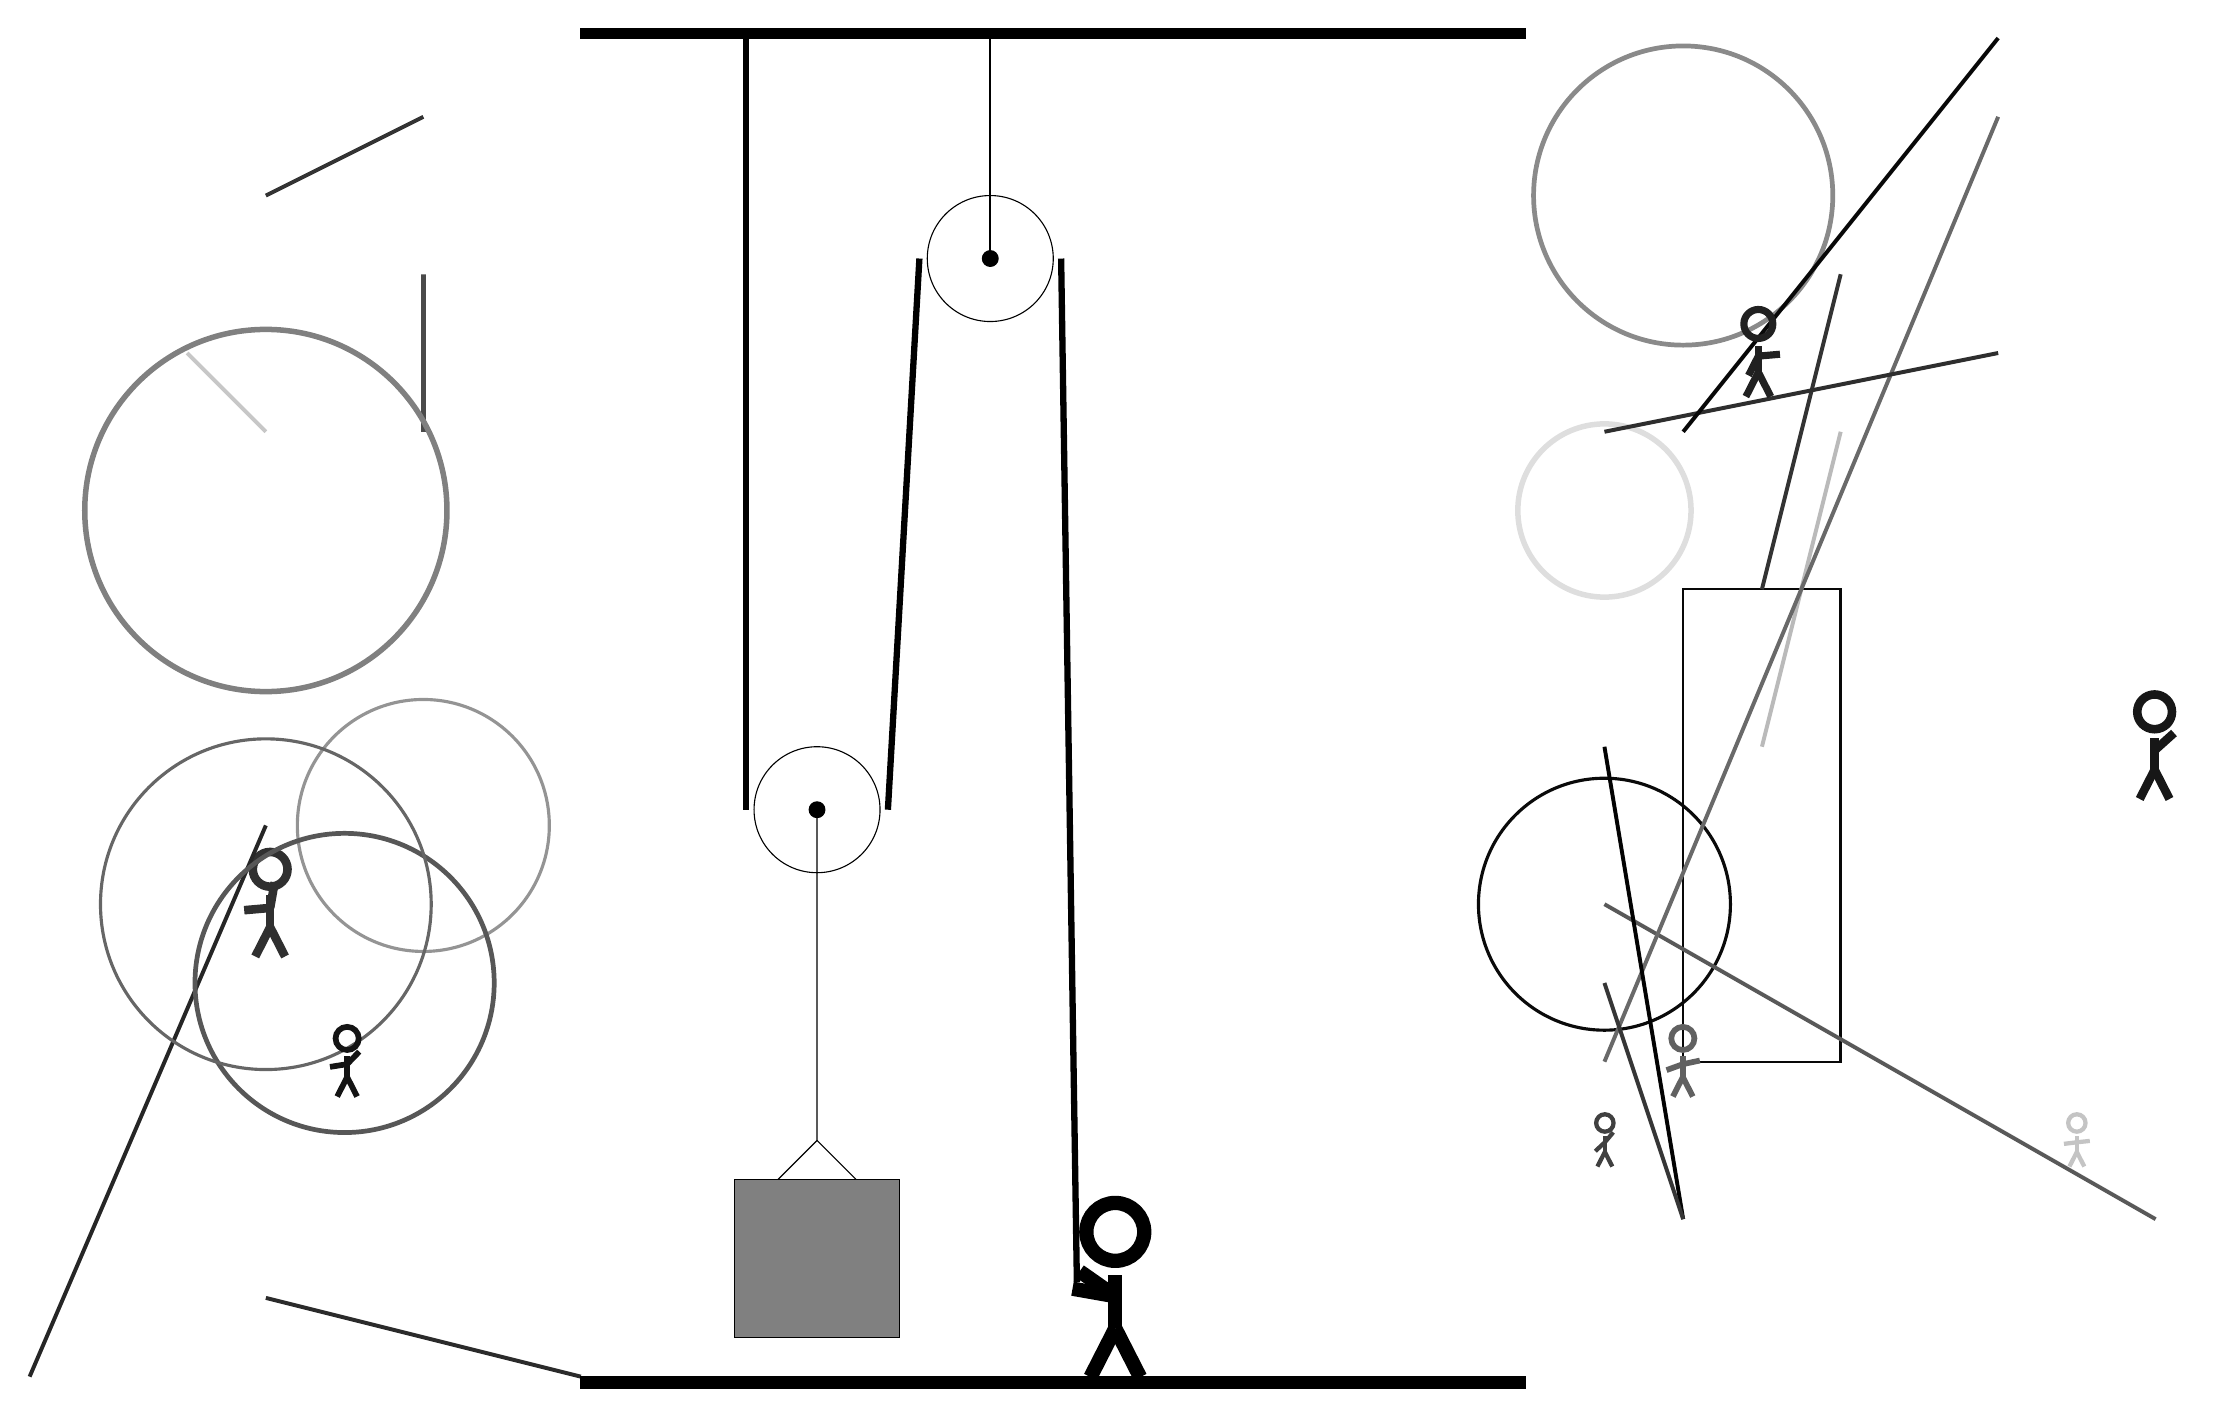
\begin{tikzpicture}
			%%%%% START %%%%%
			
			\draw[fill=black] (-2, 14) rectangle (10, 14.125);
			
			\draw (3.2, 11.2) circle (0.8);
			\draw[fill=black] (3.2, 11.2) circle (0.1);
			\draw[thick] (3.2, 11.2) -- (3.2, 14);
			
			\draw [line width=0.4mm, color=black!96](11, 3) circle (1.6);
			
			\node[line width=0.7mm, color=black!23] at (17, 0) {\Strichmaxerl[3][7][6]};
			\draw [line width=0.7mm, color=black!13](11, 8) circle (1.1);
			\draw[line width=0.3mm, color=black!97] (12, 7) rectangle (14, 1);
			\draw[line width=0.5mm, color=black!27](14, 9) -- (13, 5);
			
			\draw[line width=0.5mm, color=black!65](11, 3) -- (18, -1);
			\draw[line width=0.5mm, color=black!83](-2, -3) -- (-6, -2);
			\draw[line width=0.7mm, color=black!71] (-4, 11) rectangle (-4, 9);
			\draw[line width=0.5mm, color=black!80](13, 7) -- (14, 11);
			\node[line width=0.3mm, color=black!81] at (-6, 3) {\Strichmaxerl[6][5][80]};
			\draw[line width=0.5mm, color=black!59](11, 1) -- (16, 13);
			\draw[line width=0.5mm, color=black!85](-6, 4) -- (-9, -3);
			\draw[line width=0.5mm, color=black!99](12, -1) -- (11, 5);
			
			\draw[line width=0.5mm, color=black!80](-6, 12) -- (-4, 13);
			\node[line width=0.7mm, color=black!62] at (12, 1) {\Strichmaxerl[4][20][12]};
			\draw[line width=0.5mm, color=black!82](11, 9) -- (16, 10);
			
			\draw [line width=0.6mm, color=black!46](12, 12) circle (1.9);
			
			\node[line width=0.2mm, color=black!91] at (18, 5) {\Strichmaxerl[6][90][42]};
			\draw [line width=0.4mm, color=black!42](-4, 4) circle (1.6);
			\draw[line width=0.5mm, color=black!79](12, -1) -- (11, 2);
			\node[line width=0.4mm, color=black!75] at (11, 0) {\Strichmaxerl[3][43][50]};
			
			\draw [line width=0.6mm, color=black!66](-5, 2) circle (1.9);
			\draw[line width=0.5mm, color=black!22](-7, 10) -- (-6, 9);
			\draw [line width=0.4mm, color=black!60](-6, 3) circle (2.1);
			\draw [line width=0.7mm, color=black!50](-6, 8) circle (2.3);
			
			\draw[line width=0.5mm, color=black!97](12, 9) -- (16, 14);
			\node[line width=0.6mm, color=black!92] at (-5, 1) {\Strichmaxerl[4][9][46]};
			\node[line width=0.5mm, color=black!87] at (13, 10) {\Strichmaxerl[5][63][5]};
			
			\draw (1, 4.2) circle (0.8);
			\draw[fill=black] (1, 4.2) circle (0.1);
			
			\draw (1, 4.2) -- (1, 0) -- (0.5, -0.5);
			\draw (1, 0) -- (1.5, -0.5);
			\draw[fill=black!50] (-0.05, -0.5) rectangle (2.05, -2.5);
			
			\draw[line width=0.8mm] (0.1, 14) -- (0.1, 4.2);
			\centerarc[line width=0.8mm](1, 4.2)(180:360:0.9);
			\draw[line width=0.8mm](1.9, 4.2) -- (2.3, 11.2);
			\centerarc[line width=0.8mm](3.2, 11.2)(0:180:0.9);
			\draw[line width=0.8mm](4.1, 11.2) -- (4.3, -1.8);
			
			\node at (4.7, -1.9) {\Strichmaxerl[10][-35][170]};
			
			\draw[fill=black] (-2, -3) rectangle (10, -3.15);
			
			%%%%% END %%%%%
		\end{tikzpicture}
	\end{figure}	
\end{document}